%!TEX root = ../Dimensionieren I.tex

\section{Zug/Druck} % (fold)
	Angreifende Kraft $F_x$ im Schwerpunkt $\rightarrow$ konstantes $\sigma_x$ über den ganzen Querschnitt:
	\begin{equation*}
		\sigma_x = \frac{F_x}{A}
	\end{equation*}
	\begin{description}
		\item[Sprödbruch:] $\ang{90}$
		\item[Gleitbruch:] $\ang{45}$
	\end{description}
% section: Zug/Druck (end)
\section{Biegung} % (fold)
	Normalspannung infolge Biegung:
	\begin{equation*}
		\sigma_x = \frac{M_y}{I_y}z, \quad \sigma_{x\text{,max}}= \frac{M_y}{W_y} \qquad \text{mit}\quad W_y = \frac{I_y}{\abs{\abs{z_{\text{max}}}}}
	\end{equation*}
	$W_y$ ist das Widerstandmoment (Biegewiderstand).
	
	Axiale Flächenmomente:
	\begin{equation*}
		I_y = \int z^2 \diff A, \quad I_z = \int y^2 \diff A
	\end{equation*}
	
	Kreisquerschnitt:
	\begin{equation*}
		W_y = \frac{\pi \cdot d^3}{32}
	\end{equation*}
	
	Kreisring:
	\begin{equation*}
		W_y = \frac{\pi}{32}\cdot \frac{D^4-d^4}{D}
	\end{equation*}
% section: Biegung (end)
\section{Querkraft} % (fold)
	Schubspannung infolge Querkraft $Q_z$:
	\begin{equation*}
		\tau(z) = \frac{Q_z \cdot S_y}{I_y\cdot b}, \quad b\text{: Breite}
	\end{equation*}
	$S_y$ siehe (\ref{schubflussquerkraft}).
	
	Für den \emph{kreisrunden Querschnitt}:
	\begin{equation*}
		\tau_{zx}(z) = \frac{4Q_z}{3A}\cdot \left[ 1-\left( \frac{z}{r}\right)^2\right]
	\end{equation*}
	
	Für den \emph{rechteckigen Querschnitt}:
	\[
		\tau_{zx} = \frac{3 Q_z}{2A} \parens{1-\frac{4z^2}{h^2}}
	\]
	
	Maximal bei $z=0$.
	
% section: Querkraft (end)
\section{Torsion} % (fold)
	Schubspannung infolge Torsion:
	\begin{equation*}
		\abs{\tau_{\text{max}}} = \frac{\abs{M_t}}{W_t}, \quad \text{mit } W_t = \frac{I_p}{r_a}
	\end{equation*}
	
	Verwindung:
	\begin{equation*}
		\theta = \vartheta \cdot L , \quad \vartheta = \frac{M_t}{G\cdot I_p}
	\end{equation*}
	
	Kreisquerschnitt:
	\begin{equation*}
		W_t = \frac{\pi \cdot d^3}{16}, \quad I_p = \frac{\pi \cdot d^4}{64}=\frac{\pi \cdot r^4}{4}
	\end{equation*}
	
	Kreisring:
	\begin{equation*}
		W_t = \frac{\pi}{16}\cdot\frac{D^4-d^4}{D}, \quad I_p = \frac{\pi}{64}\cdot (D^4 -d^4)
	\end{equation*}
	Für Tabellenwerte von Trägheitsmomenten siehe Anhang \ref{torsion}.
	
	Allgemein:
	\begin{equation*}
		I_P = I_y + I_z, \quad W_y = \frac{I_y}{\abs{z_{\text{max}}}}, \quad W_p = \frac{I_p}{r_a}
	\end{equation*}
	
	Bredt-Batho-Beziehung:
	\begin{align*}
		M_t &= 2 \cdot q_0 \cdot A_0 \\
		\tau_t &= \frac{q_0}{d} = \frac{M_t}{2 \cdot A_0 \cdot d}
	\end{align*}
% section: Torsion (end)
\section{Knickbeanspruchung} % (fold)
	
	Ablauf:
	\begin{itemize}
		\item Ermittle die Schlankheit:
			\begin{align*}
				\lambda &= L_K \cdot \sqrt{\frac{A}{I}} \\
				\lambda_F &= \frac{a - R_{ed}}{b}
			\end{align*}
		\item Wähle Verfahren: \\
			\begin{tabular}{rp{5cm}}
				$\lambda > \lambda_0$: & $\Rightarrow$ Eulersche Formel \\
				$\lambda_F < \lambda < \lambda_0$: & Stab wird nicht mehr knicken, könnte aber fliessen \\[-.5ex] &
				$\Rightarrow$ Tetmajer \\
				$\lambda < \lambda_F$: & Stab wird gequetscht
			\end{tabular}
			
			\begin{equation*}
				\sigma_K = \conditional{
					\frac{\pi^2\cdot E}{\lambda^2} & \lambda > \lambda_0 \\
					a-b\lambda & \lambda_F < \lambda < \lambda_0 \text{ (vgl.~Tabelle)}
				}
			\end{equation*}
		\item Ermittle Knicksicherheit:
			\begin{align*}
				F_K &= \frac{\pi^2\cdot E \cdot I}{L_K^2} \\
				S_K &= \frac{\sigma_K \cdot A}{F_K}
			\end{align*}
	\end{itemize}

	Kritische Kraft (Euler'sche Knicklast):
	
	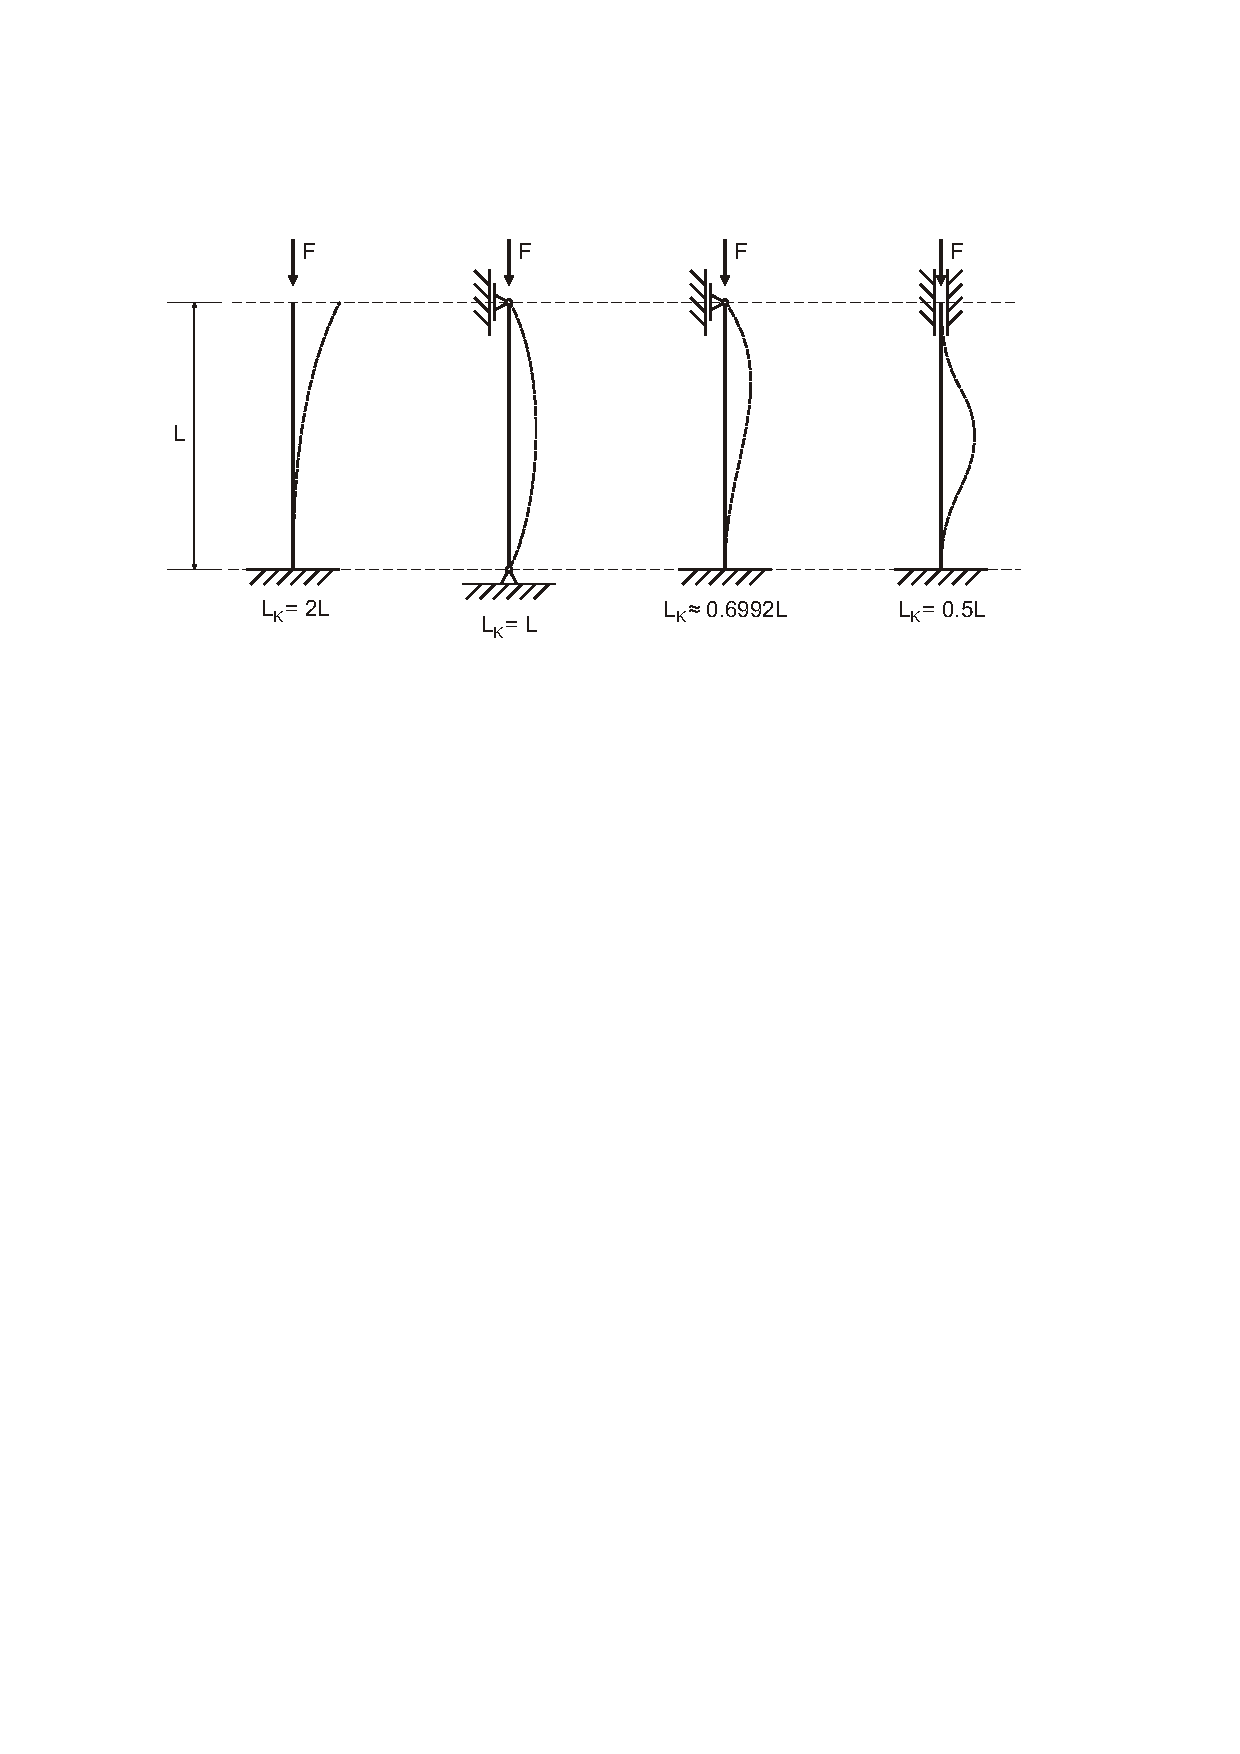
\includegraphics[width=\columnwidth]{graphics/knick}
	
	\begin{center}
		\begin{tabular}{lrrr}
			\toprule
			Werkstoff & $E$ & $\lambda_0$ & $\sigma_K \niceunit{\newton\per\Square\milli\metre}$ nach Tetmajer \\
			\midrule
			StE 255 (St37) & 210000 & 104 & $310 - 1.14\lambda$ \\
			StE 355 (St50) & 210000 & 89 & $310 -1.14\lambda$\\
			Federstahl & 210000 & 60 &$355 - 0.62\lambda$\\
			Grauguss & 115000 & 80 & $716 - 12\lambda + 0.053 \lambda^2$\\
			Nadelholz & 10000 & 100 & $29.3 - 0.194\lambda$\\
			\bottomrule
		\end{tabular}
	\end{center}
% section: Knickbeanspruchung (end)
\section{Flächenpressung} % (fold)
	\subsection{Ebene Wirkflächen} % (fold)
		\begin{equation*}
			p = \frac{F_x}{A}
		\end{equation*}
		mit $A$ als \emph{Berührungsfläche}.
	% subsection: Ebene Wirkflächen (end)
	\subsection{Zapfen-/Bohrung-Verbindung} % (fold)
		\begin{equation*}
			p = \frac{F}{A_\text{proj}} \qquad A_\text{proj} = d\cdot L
		\end{equation*}
		\vspace{-2cm}
		\begin{flushright}
			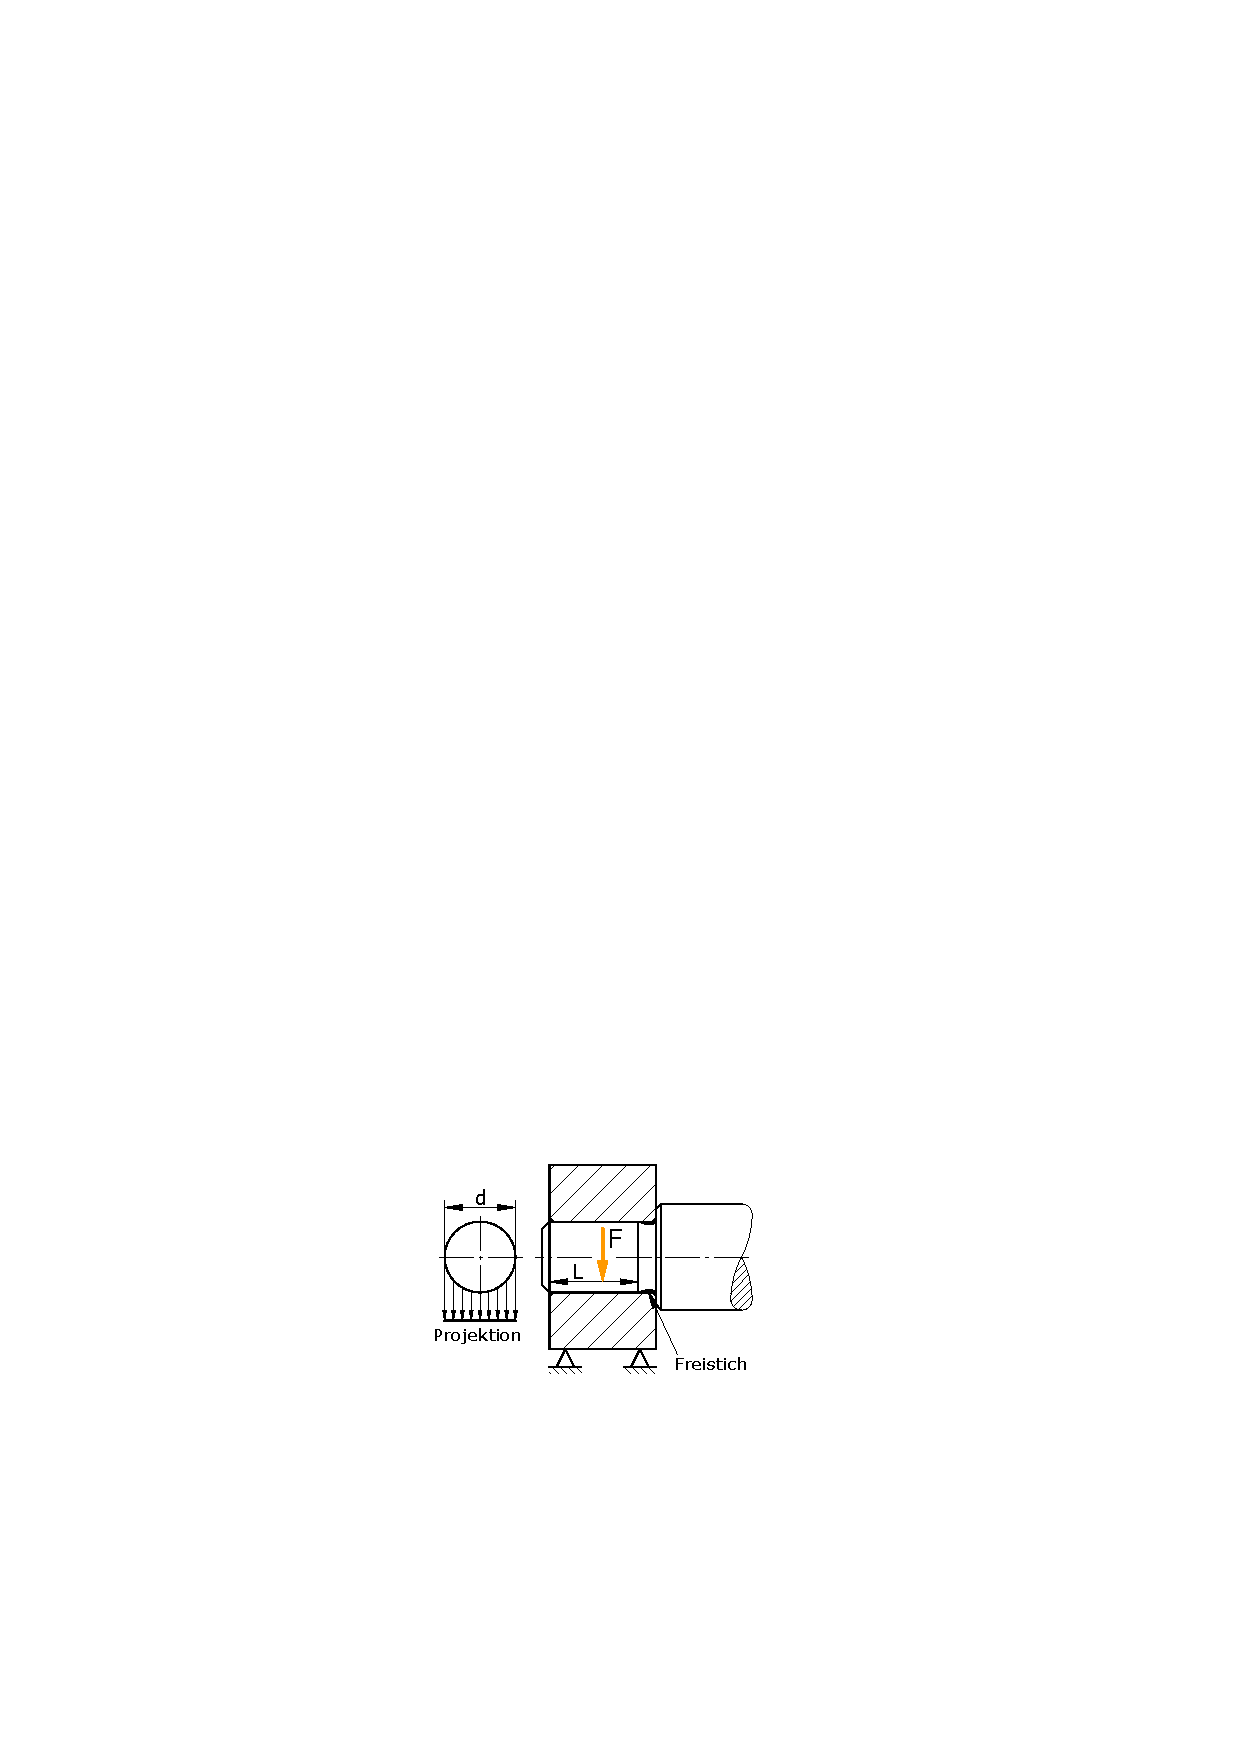
\includegraphics[width=.4\columnwidth]{graphics/lagerschale}
		\end{flushright}
	% subsection: Zapfen-/Bohrung-Verbindung (end)
	\subsection{Gewölbte Wirkflächen} % (fold)
		\subsubsection{Kugel gegen Kugel} % (fold)
			
			\begin{wrapfigure}[5]{r}{2.5cm}
				\vspace{-2cm}
				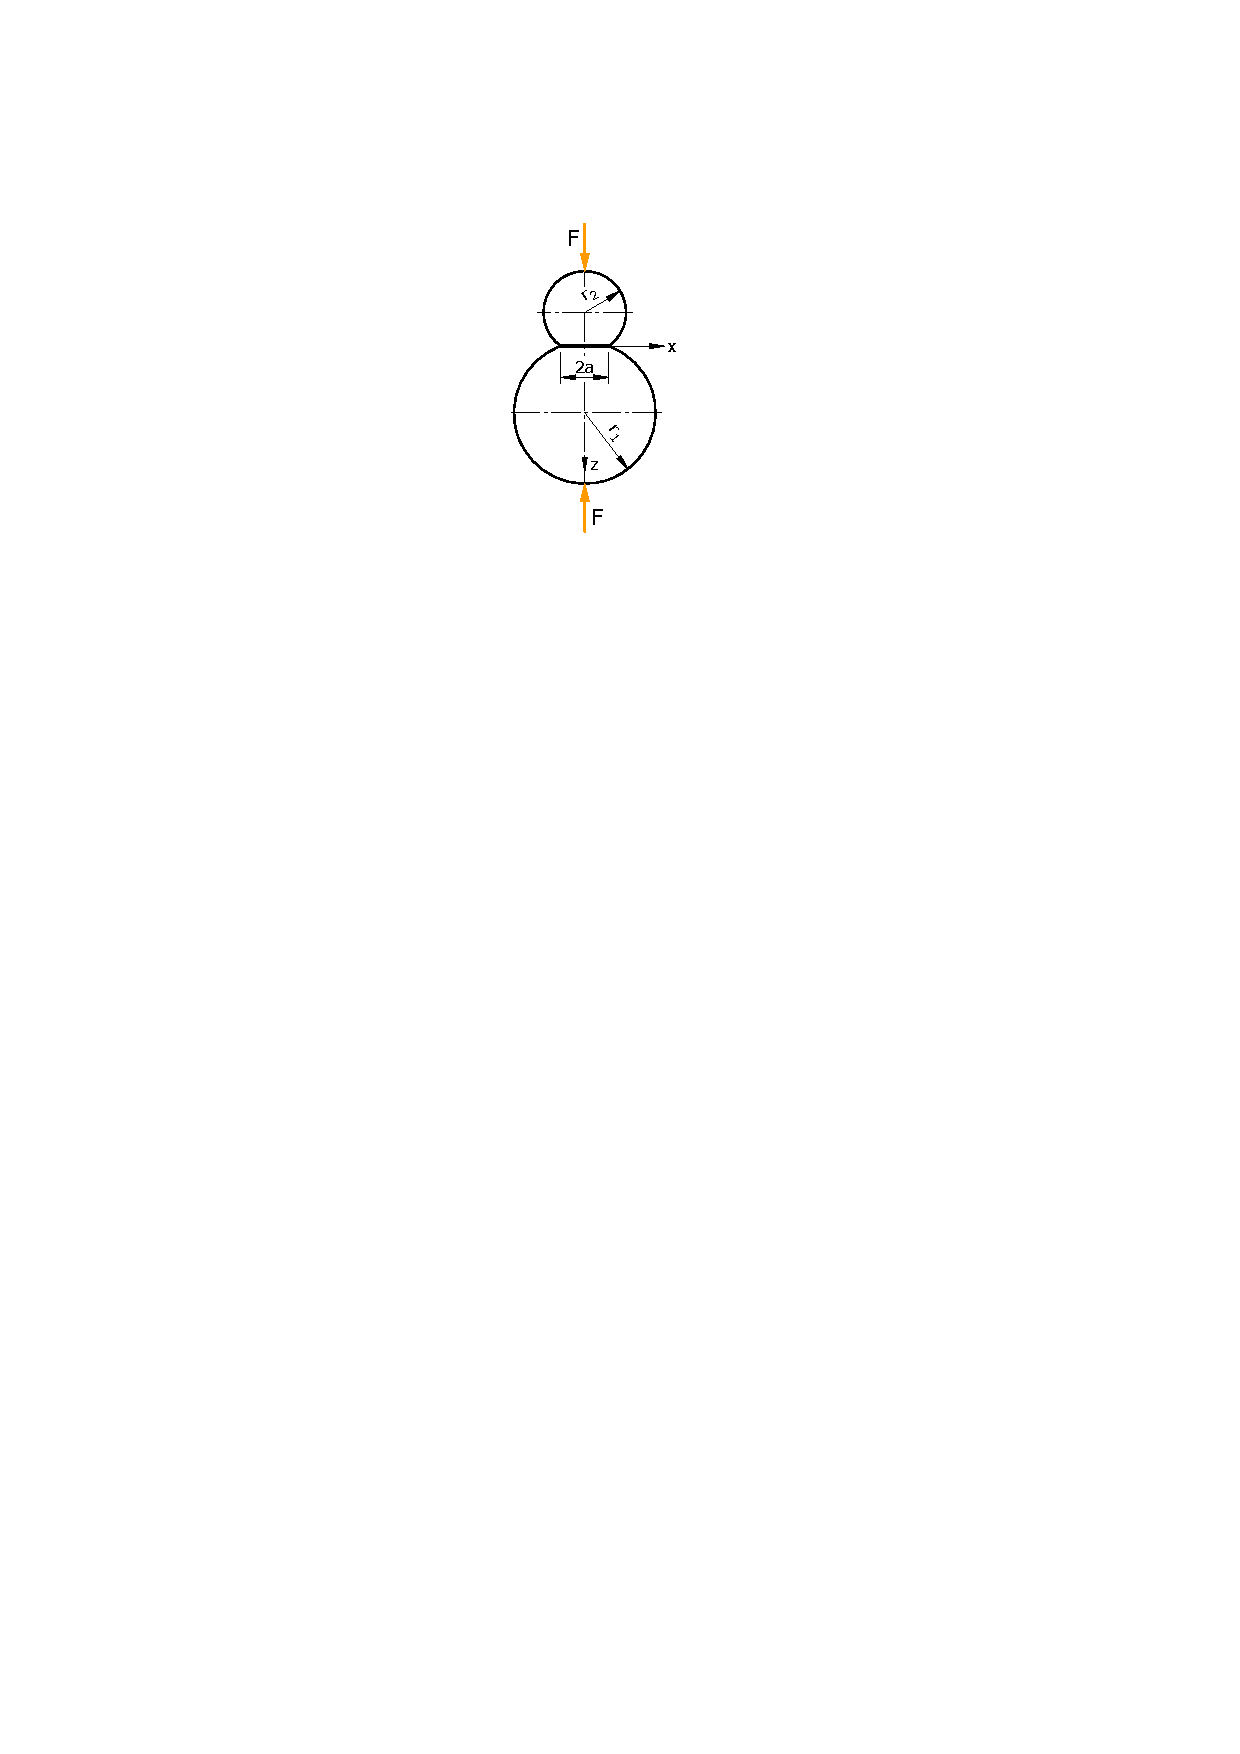
\includegraphics[scale=.8]{graphics/kugel_gegen_kugel}
			\end{wrapfigure}
		
			Druckflächenradius nach Hertz:
			\begin{equation*}
				a = \sqrt[3]{\frac{3}{4}(1-\nu^2)F\frac{\left( \frac{1}{E_1}+\frac{1}{E_2}\right)}{\left( \frac{1}{r_1}+ \frac{1}{r_2}\right)}}
			\end{equation*}
			Maximale Spannung auf der Oberfläche:
			\begin{equation*}
				p_{\text{max}}=\sqrt[3]{\frac{6F\left( \frac{1}{r_1}+ \frac{1}{r_2}\right)^2}{\pi^3(1-\nu^2)^2\left( \frac{1}{E_1}+\frac{1}{E_2}\right)^2}}
			\end{equation*}
			wobei $\nu$ die Querkontraktionszahl ist. 

			\emph{Achtung:} Radius kann unendlich (Platte) oder negativ (innere Seite einer Kugel) sein.
			\begin{equation*}
				\text{Maximale Vergleichsspannung } \sigma_\text{Vmax} = 0.62 \cdot p_\text{max}
			\end{equation*}
			\begin{equation*}
				\text{tritt auf bei } z = 0.47 \cdot a
			\end{equation*}
			
			\begin{center}
				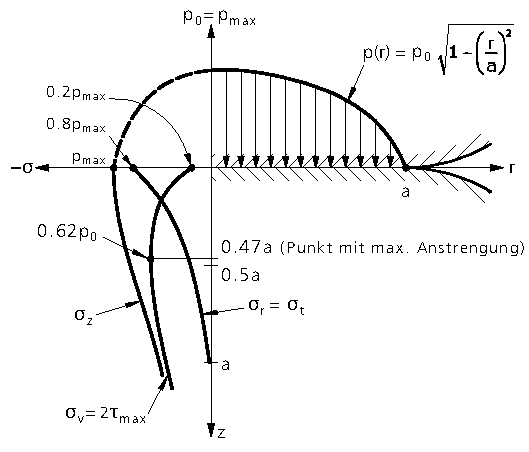
\includegraphics[width=.75\columnwidth]{graphics/kugelgraph}
			\end{center}
		% subsubsection: Kugeln (end)
		\subsubsection{Parallele Zylinder (Hertz)} % (fold)
			\begin{wrapfigure}{r}{3.55cm}
				\vspace{-1cm}
				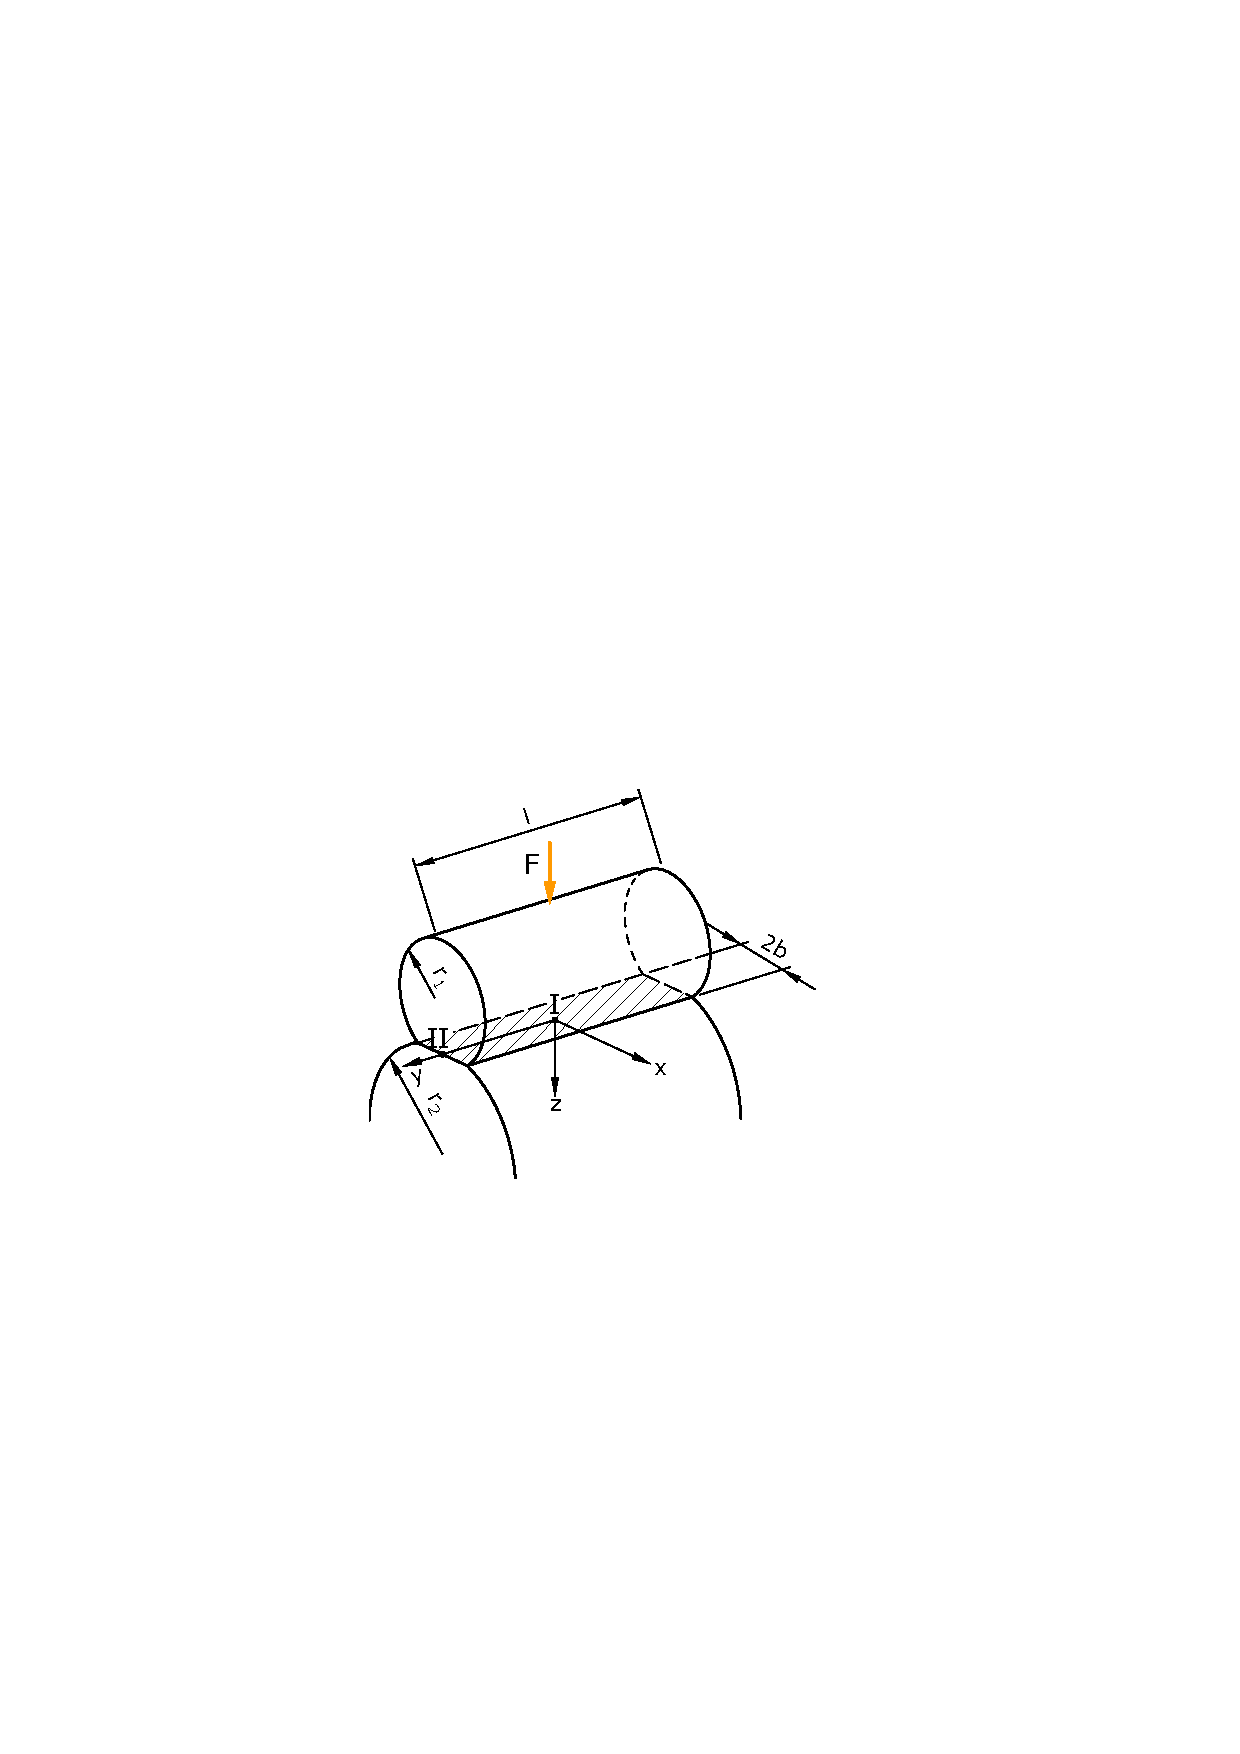
\includegraphics[scale=.525]{graphics/parallele_zylinder}
			\end{wrapfigure}
			
			Halbe Druckflächenbreite:
			\begin{equation*}
				b = \sqrt{\frac{\frac{\pi}{4}(1-\nu^2)F\left( \frac{1}{E_1}+\frac{1}{E_2}\right)}{l \cdot \left( \frac{1}{r_1}+ \frac{1}{r_2}\right)}}
			\end{equation*}
			mit $l$ Länge der Druckfläche. Maximale Pressung:
			\begin{equation*}
				p_{\text{max}}=\sqrt{
			\frac{F \cdot \left( \frac{1}{r_1}+ \frac{1}{r_2}\right)}
				{\pi (1-\nu^2) \cdot \left( \frac{1}{E_1}+\frac{1}{E_2}\right) \cdot l }}
			\end{equation*}
			Empfehlung: Abrunden / Bombieren der Kanten.
			\begin{equation*}
				\text{Maximale Vergleichsspannung } \sigma_\text{Vmax} = 0.608 \cdot p_\text{max}
			\end{equation*}
			\begin{equation*}
				\text{tritt auf bei } z = 0.78 \cdot b
			\end{equation*}
		% subsubsection: Zylinder (end)
	% subsection: Gewölbte Wirkflächen -- Kugeln (end)
% section: Flächenpressung (end)
\section{Dünnwandige Träger} % (fold)
	\subsection{Normalspannung} % (fold)
		Normalspannung infolge Biegung:
		\begin{equation*}
			\sigma_x(y,z) = \frac{M_y\cdot I_z + M_z \cdot I_{yz}}{I_y\cdot I_z - I_{yz}^2}\cdot z - \frac{M_z \cdot I_y + M_y \cdot I_{yz}}{I_y \cdot I_z - I_{yz}^2}\cdot y
		\end{equation*}
		Bei \emph{symmetrischem Querschnitt} verschwindet das Träg\-heits\-moment $I_{yz}= \int yz \cdot \diff y\diff z$, dann können wir vereinfachen:
		\begin{equation*}
			\sigma_x(y,z) = \frac{M_y}{I_y}z - \frac{M_z}{I_z}y
		\end{equation*}
		\subsection{Schubfluss infolge Querkraft}\label{schubflussquerkraft}
		\begin{equation*}
			q(s) - q_0 = -\frac{Q_y I_y + Q_z I_{yz}}{I_y \cdot I_z - I_{yz}^2}\cdot S_z(s) - \frac{Q_z I_z + Q_y I_{yz}}{I_y \cdot I_z - I_{yz}^2}\cdot S_y(s)
		\end{equation*}
		\emph{Offener Querschnitt:} $q_0$ verschwindet am Rand. \\
		\emph{Symmetrisches Profil:}
		\begin{equation*}
			q(s) = -\frac{Q_y \cdot S_z(s)}{I_z}-\frac{Q_z \cdot S_y(s)}{I_y}
		\end{equation*}
		\begin{equation*}
			S_z(s) = \int\limits_0^s t(s)\cdot y(s) \diff s \quad S_y(s) = \int\limits_0^s t(s)\cdot z(s) \diff s
		\end{equation*}
	% subsection: Normalspannung (end)
	\subsection{Schubspannungen infolge Torsion} % (fold)
		Spezifische Verdrehung:
		\begin{equation*}
			\vartheta = \frac{\theta}{L}= \frac{1}{G \cdot L} \int_0^1 \frac{M_t(x)}{I_t}\diff x = \frac{M_t}{G \cdot I_t}
		\end{equation*}
		mit $I_t$ dem Flächenträgheitsmoment bei Torsion (Saint Venant'sche Konstante), allgemein:
		\begin{equation*}
			I_t = \frac{4 \cdot \int \Phi(y,z) \diff A}{\nabla^2 \Phi(y,z)}, \quad \text{und } M_t = 2 \int_A \Phi(y,z) \diff A
		\end{equation*}
		Für Vollquerschnitt mit Annäherung an die Kreisform:
		\begin{equation*}
			I_t \approx \frac{A^4}{4\pi^2I_p}
		\end{equation*}
	% subsection: Schubspannungen infolge Torsion (end)
	\subsection{Ausgewählte Querschnitte} % (fold)
		\paragraph{Ellipse} % (fold)
			\begin{equation*}
				\Phi(y,z) = \Phi_0 \cdot \left[ \left( \frac{y}{a}\right)^2 + \left( \frac{z}{b}\right)^2 -1\right]
			\end{equation*}
		% paragraph: Ellipse (end)
		\paragraph{Rechteck} % (fold)
			\begin{equation*}
				\Phi(y,z) = \sum_m \sum_n c_{mn} \cos \left( \frac{\pi m y}{a}\right) \cos \left( \frac{\pi n z}{b}\right), \quad m,n = 1, 3, 5, \cdots
			\end{equation*}
		% paragraph: Rechteck (end)
	% subsection: Ausgewählte Querschnitte (end)
	\subsection{Torsion geschlossener Profile} % (fold)
		Schubfluss ist konstant $q = q_0 = \text{const.}$. Für zylindrische Stäbe mit geschlossenem Querschnitt gilt:
		\begin{equation*}
			M_t = 2 \cdot q_0 \cdot A_0 = F \cdot I_t \cdot \vartheta, \text{mit } I_t = \frac{4 A_0^2}{\oint_s \frac{\diff s}{t(s)}}
		\end{equation*}
	% subsection: Torsion geschlossener Profile (end)
% section: Dünnwandige Träger (end)
\section{Achsen und Wellen} % (fold)
	\subsection{Verformung infolge Torsionsbeanspruchung} % (fold)
		\begin{equation*}
			\vartheta = \frac{\theta}{L} = \frac{M_t}{G \cdot I_p}
		\end{equation*}

		Verdrehungswinkel in Grad:
		\begin{align*}
			\theta &= \frac{180}{\pi} \frac{M_t L}{G I_p} = 584 \cdot \frac{M_t L}{G d^4} \\
			\theta_\text{Ges} &= \frac{584}{G} \sum_i \frac{M_{ti} L_i}{d_i^4}
		\end{align*}
		Der Gesamtverdrehungswinkel ergibt sich aus der Summe der einzelnen Wellenabschnitten.
	% section: Verformung infolge Torsionsbeanspruchung (end)
	\subsection{Verformung infolge Biegebanspruchung} % (fold)
		\begin{equation*}
			w''(x) = -\frac{M_b(x)}{E\cdot I_y(x)}
		\end{equation*}
		
		\paragraph{Ermittlung der Durchbiegung und Neigung einer zweifach gelagerten Welle} % (fold)
			Die Welle wird an der Stelle durchgeschnitten, wo die Durchbiegung bestimmt werden soll.
			
			\hspace{-.0625\columnwidth}
			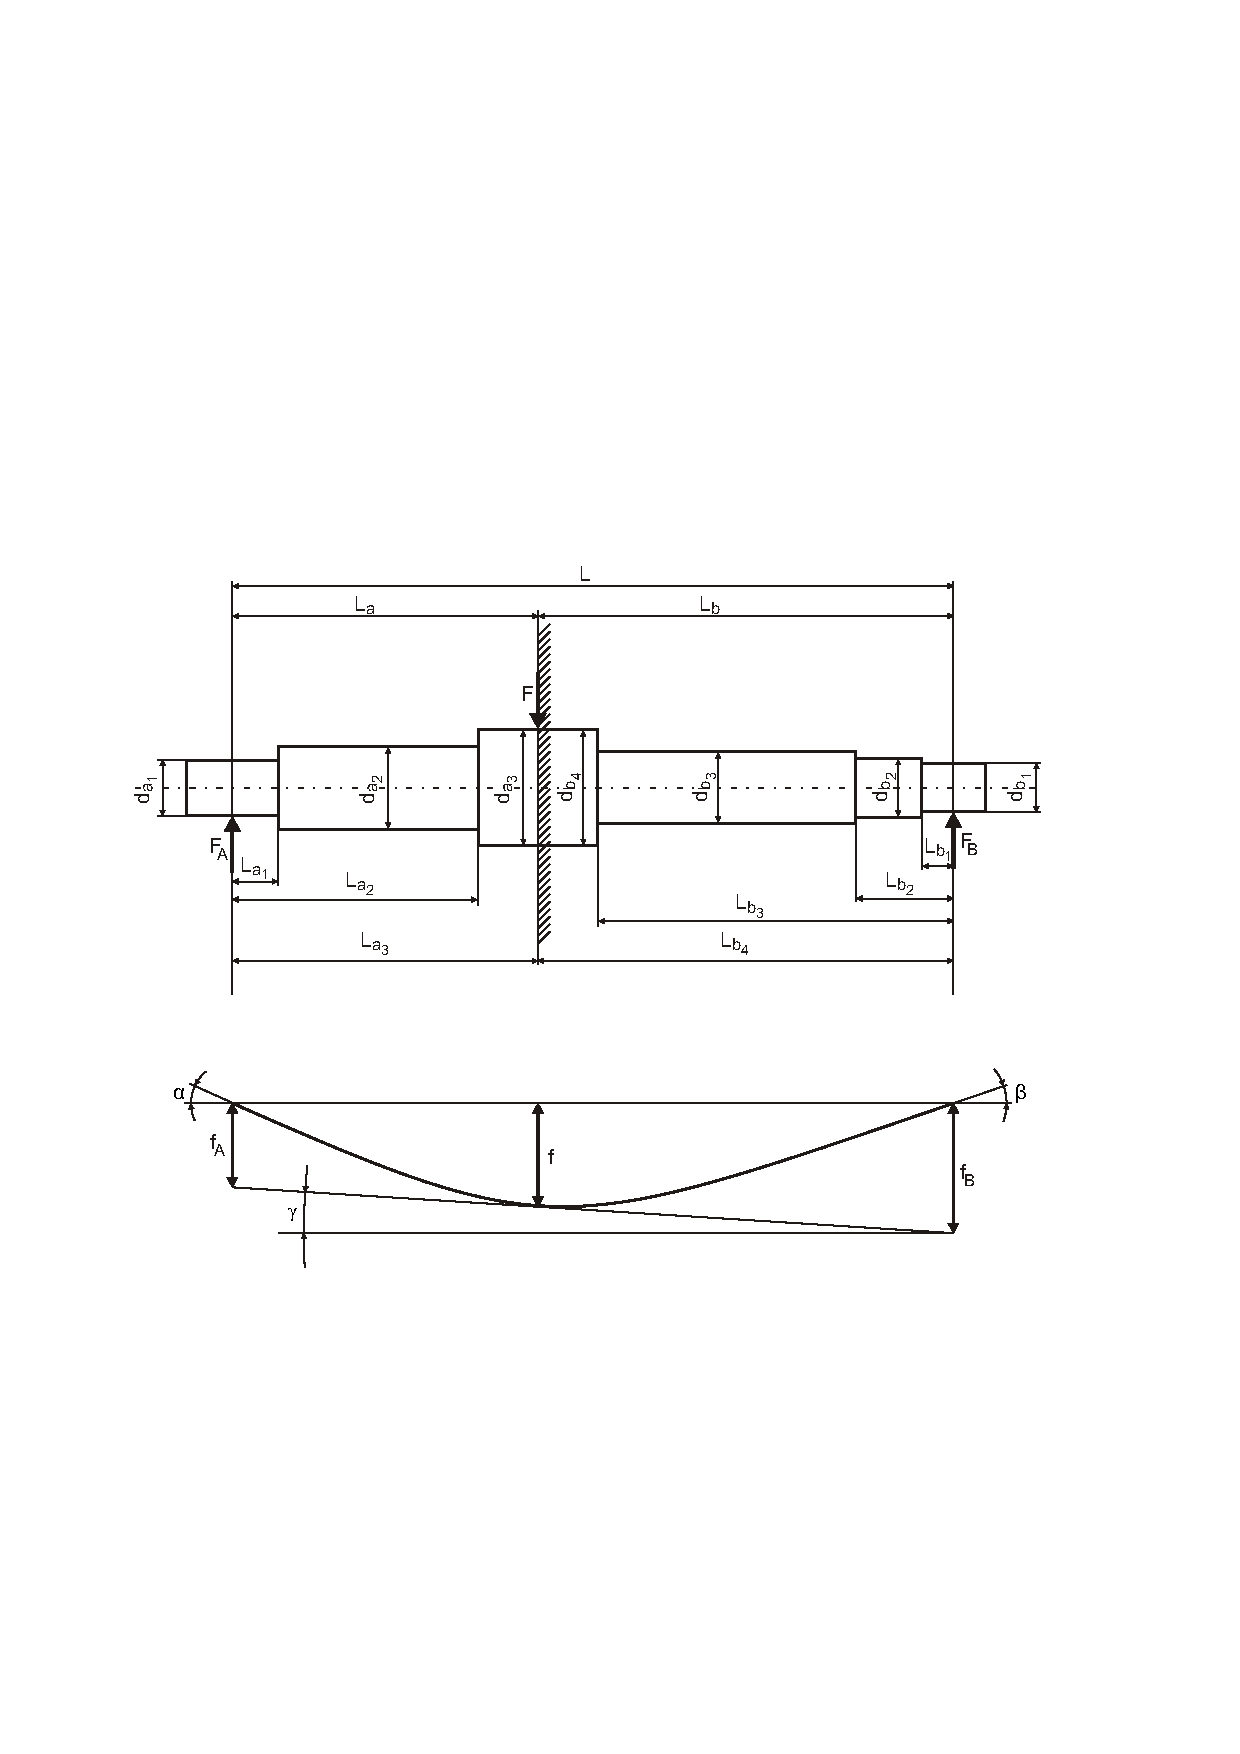
\includegraphics[width=1.1\columnwidth]{graphics/welle_durchbiegung}
			
			\begin{align*}
				f &= \frac{F L^3}{3 E I}\sunit{\mm}\,,\qquad I = \frac{\pi d^4}{64} \\[1ex]
				f_A &= \frac{F_A}{3E} \parens{
					\frac{L_{a_1}^3}{I_{a_1}} + \frac{L_{a_2}^3 - L_{a_1}^3}{I_{a_2}} + \frac{L_{a_3}^3 - L_{a_2}^3}{I_{a_3}}
				} \\[1ex]
				\tan \alpha \approx \alpha &= \frac{F_A}{2E} \parens{
					\frac{L_{a_1}^2}{I_{a_1}} + \frac{L_{a_2}^2 - L_{a_1}^2}{I_{a_2}} + \frac{L_{a_3}^2 - L_{a_2}^2}{I_{a_3}}
				} \\[1ex]
				f &= f_A + \frac{L_a}{L}(f_B - f_A) \\[1ex]
				\tan \gamma \approx \gamma &= \frac{f_A - f_B}{L}
			\end{align*}
			
			$f_B$ berechnet sich analog zu $f_A$. Die Neigung $\alpha L$ am Lager $A$ und $\beta_L$ am Lager $B$ sind:
			\begin{equation*}
				\alpha_L = \alpha - \gamma \qquad \beta_L = \beta + \gamma
			\end{equation*}
		% paragraph: Ermittlung der Durchbiegung und Neigung einer zweifach gelagerten Welle (end)
	% section: Verformung infolge Biegebanspruchung (end)
	\subsection{Bestimmung der kritischen Drehzahl und Winkelgeschwindigkeit} % (fold)
		Kritische Winkelgeschwindigkeit und Drehzahl mit der Durchbiegung $f_G$:
		\begin{align*}
			\omega_k &= 99 \sqrt \frac{1}{f_G} \nicesunit{\per\second} \\
			n_k &\approx 946 \sqrt{\frac{1}{f_G}}
		\end{align*}
	% subsection: Bestimmung der kritischen Drehzahl (end)
	\subsection{Vorgehen bei mehreren Einzelmassen} % (fold)
		Bei mehreren Einzelmassen muss für die Bestimmung der einzelnen $\omega_k$ nur jeweils eine Gewichtskraft berücksichtigt werden.
		
		Hat eine Welle also zwei Massen, so müssen $f_A$ und $f_B$ zweimal bestimmt werden, indem eine Masse jeweils entfernt wird. Dies resultiert in unterschiedlichen Lagerkräfte.
		
		Die niedrigste kritische Winkelgeschwindigkeit der ganzen Welle $\omega_k$ für eine zweifach gelagerte Welle mit mehreren Drehmassen ist dann:
		\begin{equation*}
			\frac{1}{\omega_k^2} = \frac{1}{\omega_{k0}^2} + \frac{1}{\omega_{k1}^2} + \cdots + \frac{1}{\omega_{kn}^2}
		\end{equation*}
	% subsection: Vorgehen bei mehreren Einzelmassen (end)
% section: Achsen und Wellen (end)

\section{Zahnräder} % (fold)
	\[
		L = M\cdot \omega = F_t \frac{d}{2} \cdot 2\pi n
	\]
% section: Zahnräder (end)